%--------------------------------------------------------------------------------------------------------------------
%------------------------------------------------- Chapter 5 --------------------------------------------------------

\chapter{Framework para la inyección de contratos sensibles al contexto en
entornos Web colaborativos} \label{cap:framework} \label{cap:6}
%\chapter{Framewrok to Implemet Context Aware Contract in E-learning

%\pagenumbering{arabic}


\section {Introducción} \label{intro}

A medida que el avance en la investigación y desarrollo de plataformas
e-learning brindan mejoras e innovaciones en herramientas
(videoconferencias, porfolios, wikis, workshops, etc.) y sus respectivos
servicios, crece la cantidad de posibles configuraciones de los espacios
e-learning. Estas configuraciones abarcan diferentes tipos de requerimientos
pertenecientes a las etapas de diseño, desarrollo e incluso exigen que el
espacio e-learning se adapte en tiempo de ejecución. A partir de estos
requerimientos se definen los procesos e-learning (que nosotros denominamos
Pe-lrn) \cite{tweb} de manera semejante a procesos de negocio en otro dominio de
aplicación. Al igual que los procesos de negocios en una Aplicación Web
convencional, los Pe-lrn están compuestos por transacciones Web \cite{}. En este
contexto, una transacción (o transacción e-learning) es definida como una
secuencia de actividades que un usuario ejecuta a través de una Aplicación
e-learning con el propósito de efectuar una tarea o concretar un objetivo, donde
el conjunto de actividades, sus propiedades y las reglas que controlan sus
ejecuciones dependen del Pe-lrn que la Aplicación debe brindar. Un ejemplo de
estrategia didáctica es la posibilidad de que un alumno acceda a determinado
tipo de material (vídeos, archivos, etc.)  dependiendo de sus intervenciones en
los Foros. Estos tipos de requerimientos resultan difíciles de implementar con
las actuales aplicaciones e-learning de extendido uso a nivel global. 

%Un ejemplo de un objetivo pedagógico es la posibilidad de que un alumno acceda a determinado tipo de material (vídeos, archivos, etc.)  dependiendo de sus intervenciones en los Foros. Este tipo de requerimientos son difíciles de implementar con las aplicaciones e-learning actuales \cite{libro}.

Las características funcionales de las actuales aplicaciones Web e-learning
(AWe-lrn), como Sakai\footnote{SaKai: Entorno colaborativo y de aprendizaje para
enseñar. Es de código abierto y está resuelto con tecnología Java. Véase
detalles en  \homedir{wwww.sakaiprojet.org})}, se basan en brindar navegación
entre páginas a través de links y ejecución de transacciones e-learning por
desde las herramientas (ej., Foros, Anuncios, Exámenes, Blogs, etc.) que
utilizan los servicios de la plataforma (ej., edición, manejo de audio y vídeo,
consultas, navegación, etc.). %La forma en que estos servicios son implementados
y la forma en que sus configuraciones pueden ser alteradas, son actualmente un
fuerte impedimento para implementar requisitos como el mencionado anteriormente.
%La configuración de estos servicios está fuertemente ligada a los aspectos
tecnológicos involucrados en las etapas de diseño y, principalmente, en la etapa
de desarrollo e implementación.% 

En el marco de los análisis efectuados podemos sostener que el proyecto Sakai
brinda una de las propuestas más consolidadas de diseño y desarrollo de entornos
colaborativos e-learning para educación, orientado a herramientas que se
implementan a través de servicios comunes (servicios bases). Por ejemplo, el
servicio de edición de mensajes es utilizado en las herramientas Foro, Anuncio,
Blog, PorFolio, etc. Más aun, otras de las características salientes de Sakai es
la versatilidad para su extensión y/o configuración. En efecto, Sakai permite
alterar ciertas configuraciones en tiempo de ejecución, por ejemplo,
instrumentar una nueva funcionalidad en un servicio base de Sakai. 


Sin embargo,  estas soluciones no pueden resolver aquellos Pe-lrn que involucren
cambios en el comportamiento de la relaciones entre un componente (cliente) que
ocasiona, a través de un pedido, la ejecución de un componente servidor
(proveedor). Estos tipos de cambios refieren a la capacidad de adaptación
dinámica del sistema \cite{kcomponent} extendiendo, personalizando y mejorando
los servicios sin la necesidad de recompilar y/o reiniciar el sistema. En este
trabajo se presenta un propuesta para la incorporación (agregado) de propiedades
de adaptación dinámicas a los servicios bases del framework Sakai, especialmente
diseñadas para implementar Pe-lrn definidos en el marco de \cite{ob} donde se
requieren nuevos aspectos de adaptación \cite{libro} en la perspectiva de los
Dispositivos Hipermediales Dinámicos en el campo del e-learning \cite{maxi} con
característica \textit{context-aware} \cite{libro5,libro6}. Se entiende por DHD
\textit{``a una red social mediada por las TIC en un contexto
físico-virtual-presencial, donde los sujetos investigan, enseñan, aprenden,
dialogan, confrontan, evalúan, producen y realizan responsablemente procesos de
transformación sobre objetos, regulados según el caso, por una coordinación de
contratos integrados a la modalidad participativa del Taller''}. (San Martín et
al, 2008) 

%Nuestra propuesta consite en lograr los niveles de flexibilidad dinámica mencionado incorporando a Sakai un framework para la coordinación de contratos. 


El resto de este trabajo se encuentra organizado de la siguiente manera:
Tras esta introducción se presenta una referencia conceptual del framework
contratos con características ``context-aware``, utilizados en el proyecto Obra
Abierta: Dispositivos Hipermediales Dinámicos para educar e investigar (Dir.
Dra. Patricia S. San Martín (Sección \ref{contrato}). Luego se describe la
macro-arquitectura de integración entre los frameworks de Sakai, la teoría de
coordinación de contratos sensible al contexto (TCCs-c), un modelo de contratos
context-aware y aplicaciones externas (sección \ref{macro}). Siguiendo,
se presenta un modelo de implementación de la TCCs-c a través del de patrones de
diseño (sección \ref{patron}). En la sección \ref{caso de estudio} se propone un
caso de estudio concreto. Finalizando con una
breve conclusión.


\section{Contractos con características sensibles al contexto} \label{contrato}

Nuestra propuesta de solución a los requerimientos mencionados sobre adaptación
dinámica comienza con la construcción de un modelo de contrato orientado a la
implementación de servicios sensibles al contexto. El uso de contratos parte de
la noción de Programación por Contrato ("Programing by Contract") de Meyer
\cite{Meyer} basada en la metáfora de que un elemento de un sistema de software
colabora con otro, manteniendo obligaciones y beneficios mutuos. En nuestro
dominio de aplicación consideraremos que un objeto cliente y un objeto servidor
``acuerdan`` a través de un contrato (representado con un nuevo objeto) que el
objeto servidor satisfaga el pedido del cliente, y al mismo tiempo el cliente
cumpla con las condiciones impuestas por el proveedor. Como ejemplo de la
aplicación de la idea de Meyer en  nuestro dominio de sistemas e-learning
planteamos la situación en que un usuario (cliente) utiliza un servicio de
edición de mensajes (servidor) a través de un contrato que garantizará las
siguiente condiciones: el usuario debe poder editar aquellos mensajes que tiene
autorización según su perfil (obligación del proveedor y beneficio del cliente);
el provedor debe tener acceso a la información del perfil del usuario
(obligación del cliente y beneficio del proveedor).

A partir de la conceptualización de contratos según Meyer se propone una
extensión por medio del agregado de nuevas componentes para instrumentar
mecanismos que permitan ejecutar acciones dependiendo del contexto. 

En aplicaciones sensibles al contexto \cite{Dey}, el contexto (o información de
contexto) es definido como la información que puede ser usada para caracterizar
la situación de una entidad más allá de los atributos que la definen. En nuestro
caso, una entidad es un usuario (alumno, docente, etc.), lugar (aula,
biblioteca, sala de consulta, etc.), recurso (impresora, fax, etc), u objeto
(examen, trabajo práctico, etc.) que se comunica con otra entidad a través del
contrato. En \cite{libro5} se propone una especificación del concepto de
contexto partiendo de las consideraciones de Dourish \cite{contexto} y adaptadas
al dominio e-learning, que será la que consideraremos en este trabajo. Contexto
es todo tipo de información que pueda ser censada y procesada, a través de la
aplicación e-learning, que caracterizan a un usuario o entorno, por ejemplo:
intervenciones en los foros, promedios de notas, habilidades, niveles de
conocimientos, máquinas (direcciones ip) conectas, nivel de intervención en los
foros, cantidad de usuarios conectados, fechas y horarios, estadísticas sobre
cursos, etc.


En términos generales, la coordinación de contratos es una conexión
establecida entre un grupo de objetos aunque en este trabajo se consideran sólo
dos objetos: un cliente y un servidor.



Cuando un objeto, cliente efectúa una llamada a un objeto servidor (ej.,
elservicio de edición de la herramienta Foro), el contrato ''intercepta'' la 
llamada y establece una nueva relación teniendo en cuenta el contexto del objeto
cliente, el del objeto servidor, e información relevante adquirida y
representada como contexto del entorno \cite{contexto}. Como condición
necesaria, el uso de  contratos no debe alterar la funcionalidad de     
la implementación de los objetos participantes, aunque sí se espera que altere
la funcionalidad del sistema.

A continuación se presenta un modelo conceptual resumido de contratos sensibles
al contexto. Se brindarán detalles sobre algunas de los componentes y relaciones
esenciales para la integración de este modelo con el framework Sakai y con los
módulos que instrumentan la coordinación de contratos \ref{macro}.

\subsection {Elementos de los contratos sensibles al contexto}

% %El contrato puede ser configurado por medio de diferentes mecanismos, desde el
% lenguaje cotidiano hasta un lenguaje de especificación formal, o un lenguaje
% basado en XML para los casos que sean necesarias especificaciones que puedan ser
% procesadas por máquinas. 

Un contrato que siga las ideas de Meyer contiene contiene toda la información
sobre los servicios que utilizarán los clientes.Para incorporar sensibilidad al
contexto nuestros contratos deberán tener referencias sobre algún tipo de
información de contexto para su utilización.

En el diagrama de relaciones entre entidades mostrado en la Figura
\ref{contratoca} se describen los elementos que componen elconcepto de contrato
sensible al contexto, especialmente para Pe-lrn.

\begin{figure}[!ht]
\begin{center}
	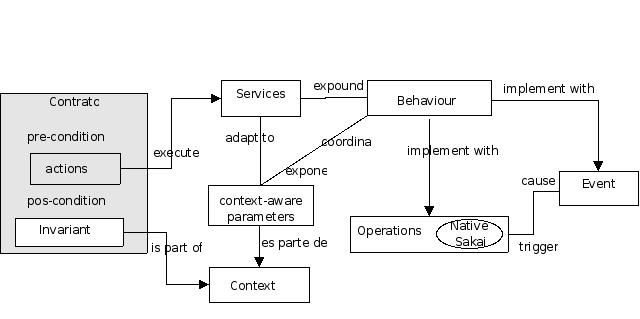
\includegraphics[width=5 in,totalheight=2.8 in]{Ch5/f1}
	\caption{\small \sl Modelo de un contrato context-aware} \label{contratoca}
\end{center}
         \end{figure}

El propósito de la presentación de este modelo de contrato sensible al contexto es identificar cuales son los componentes que lo componen y que serán referenciados en la siguiente sección para la implementación de un modelo de integración con el framework Sakai. 

La figura comienza con la representación de un contrato según Meyer donde se caracterizan los principales elementos que lo componen (pre-condiciones, acciones, pos-condiciones). La flechas salientes de la zona gris indican los dos tipos de relaciones que se debe instrumentar para incorporar un mecanismo que provea a los contratos la característica de sensibilidad al contexto. La primera de estas relaciones indica que desde las acciones del contrato se invocan a los servicios que provee un objeto servidor. La segunda relación se da debido los invariantes pueden depender de información de contexto. En la porción derecha de la Figura \ref{contratoca} aparecen las entidades necesarias para obtener contratos sensibles al contexto. Las explicamos a continuación.  

\begin{description}
\item[Servicios:] En esta componente se representan los elementos necesarios para la identificación de un servicios y clasificación de los servicios que pueden formar parte de las acciones de los contratos. Por ejemplo, nombre del servicio, identificadores, alcance, propósito, etc. Para más detalles consultar \cite{libro6}. El comportamiento funcional de cada servicio se expone a través de la componente \textbf{Comportamiento}.

\item[Comportamiento:] El comportamiento de un servicio se logra a partir de combinar operaciones y eventos que son representadas con el las componente \textbf{Operaciones} y \textbf{Eventos}. De la misma manera el servicio puede ser implementado a través del uso de eventos, representados con el componente \textbf{Eventos}, que puede lanzado operaciones del componente \textbf{Operaciones}. Por ejemplo, de acuerdo con los roles (ej., alumno, instructor, docente, etc.) asignados a un usuario de una herramienta involucrado en un Pe-lrn, en un determinado contexto del entorno (ej., si está en un espacio Foro) y del usuario (ej., si tiene permiso de moderador), la componente \textbf{servicio} brindan distintas funcionalidades (ej., editar un mensaje), que son instrumentadas por medio de operaciones concretas (ej., guardar un mensaje en una tabla) y/o a través de la publicación o subscripción de eventos. Las operaciones pueden ser de dos tipos: operaciones
que cambian el estado del sistema (tipo “update”) y/o operaciones que
proveen algún tipo de información sobre consultas  (tipo “query”). Estas operaciones pueden ser creadas creadas por el programador o utilizadas a partir de las operaciones provista por el núcleo del framework sakai (ej., adquirir el id de un canal de mensajes) usadas en los servicios bases (ej., el servicio de edición de mensajes). 

\item [Parámetros Context-Aware:] Se denomina \textbf{parámetros context-aware} a la representación de la información de contexto que forma parte de los parámetros de entrada de las funciones y métodos exportados por los servicios, estableciendo de esta manera una relación entre el componente \textbf{Servicios} y el componente \textbf{Parámetros contex-aware}. La influencia de estos parámetros en el comportamiento funcional de los servicios es representada a través de la relación entre los componentes \textbf{Parámetros context-aware} y  \textbf{Comportamiento}. 

\item[Contexto:] Este componente representa el contexto o información de contexto definida anteriormente en esta sección. Para nuestro modelo este tipo de información es utilizada de dos maneras diferentes: en primer lugar para la asignación de los valores que toman los \textbf{Parámetros context-aware}; en segundo lugar esta información puede ser utilizada para definir los invariantes que se representan en los contratos.
\end{description}



\section {Modelo de integración de Sakai con contratos} \label{sec:integracion} \label{macro} 

En esta sección se muestra un esbozo de la propuesta para incorporar a Sakai un mecanismo de coordinación de contratos sensibles al contexto, a través de la presentación de una diseño que describe la comunicación entre módulos \cite{arqModulos} y sus dependencias. En la figura \ref{macroarquitectura} los módulos son representados con paquetes UML y las relaciones  entre ellos por medio de flechas que indican comunicación y  dependencias. A su vez, en un segundo plano se muestra cuáles son las clases específicas de cada módulo y cómo se implementa la integración a través de estas.


El framework Sakai, representado en la figura \ref{macroarquitectura} por el módulo Sakai, está diseñado según una arquitectura de cuatro capas \cite{arquitectura}: La capa de \textbf{agregación} se encarga completamente de la  implementación de la interfaz con el usuario al estilo de las implementaciones de portales Web. La segunda capa denominada \textbf{presentación} tiene la responsabilidad de permitir la reutilización de los componentes Web (ej., "widget" que proveen calendarios, editores "WSYWIG", etc.). La tercera corresponde a la capa de \textbf{herramientas} donde reside la lógica de negocio de las herramientas Sakai que interactúan con el usuario (ej., Foro, Wiki, etc.). Por último la capa de \textbf{servicio} implementa los servicios Sakai bajo una Arquitectura Orientada a Servicios que serán utilizados por varias herramientas a través de API. 

Para nuestra propuesta de integración tendremos en cuenta únicamente servicios que componen laa capa de \textbf{servicios} pertenecientes a los servicios bases Sakai. Los servicios del núcleo Sakai serán envueltos mediante la coordinación de contratos, lo que se representa en la Figura \ref{macroarquitectura} con las referencias del \textbf{Módulo Sakai} hacia el \textbf{Módulo de Coordinación de Contractos}.


De esta forma, se logra controlar las invocaciones a los servicios del núcleo Sakai a través del \textbf{módulo} \textbf{Coordinación de Contratos}, quedando establecida una primer relación de integración. Esta misma relación es implementada a nivel de clases como una relación de agregación entre la clase \textit{Servicios Sakai} (correspondiente al módulo Sakai) y la clase \textit{Conector} correspondiente al framework de coordinación que será tratado en la sección \ref{patron} a través del uso de patrones de diseño.

\begin{figure}[!ht]
\begin{center}
	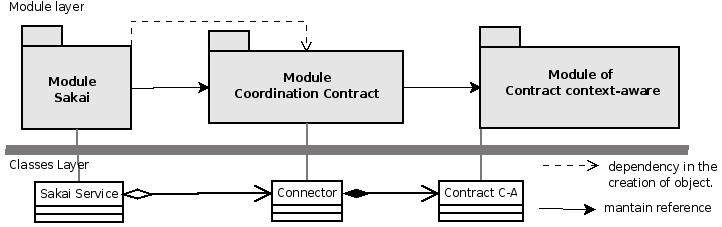
\includegraphics[width=4.5 in,totalheight=2.4 in]{Ch5/f2}
	\caption{\small \sl Diseño de la integración de Sakai con Contratos} \label{macroarquitectura}
\end{center}
\end{figure}

La última relación de integración se produce entre el módulo de \textbf{Coordination de Contratos } y el módulo de \textbf{Contratos Sensible al contexto} el cual fue  desarrollado en la sección \ref{contrato}. En este caso, la figura \ref{macroarquitectura} muestra cómo desde el framework de coordinación se estable una relación de composición entre la clase \textit{Conector} y la clase \textit{Contrato C-A} que implementa el elemento Contrato representado en la Figura \ref{contratoca} coloreada en gris.

De esta forma, instanciando dinámicamente diferentes contratos, Sakai presentará una flexibilidad en tiempo de ejecución que actualmente no posee y que es la que requieren los DHD. 
 

\section{Implementación de contratos en Sakai} \label{patron}

En las secciones anteriores se mencionó al contrato como un agente activo que se encarga de la coordinación de las componentes que lo integran. En esta sección se describe cómo este mecanismo fue implementado a través de una herramienta que permite modificar implementaciones de clases Java de los servicios Sakai para incorporarle mecanismos de coordinación de contratos sensibles al contexto, según el diseño mostrado en la Figura \ref{macroarquitectura}. Sin embargo creemos que antes es conveniente resumir brevemente otros intentos de proveer la flexibilidad requerida por los DHD.

Lograr este grado de flexibilidad es absolutamente necesario teniendo en cuenta que la implementación de estas clases, para los frameworks colaborativos e-learning como Sakai, no pueden ser modificadas (rediseñadas, reemplazadas). Para estos casos, la implementación de la TCCs-c proporciona un mecanismo que se distingue de propuestas existentes para el modelado de interacción entre objetos. 

\subsection {Niveles de flexibilidad de Sakai}

Diferentes estándares y frameworks de desarrollo de software basados en componentes e inyección de servicios fueron propuestos para mejorar la flexibilidad y adaptabilidad\footnote {La adaptabilidad en el sentido que se proponen en los sistemas hipermediales que permiten personalizarse (adaptarse) en función de los usuarios individuales (Henze, 2000).} de los sistemas e-learning Web, los más importantes son: CORBA, JavaBeans, Hibernate, Spring, JSF, RSF, etc. Sin embargo, ninguno de estos estándares proveen un mecanismo convenientemente implementativo y abstracto en donde se 
permita representar a las relaciones entre usuarios y servicios como un objeto de primera clase \cite{Meyer}. En este sentido, se implementa una solución utilizandos patrones de diseño que implemente características deseadas de la TCCs-c sobre la capa de servicios base de framework Sakai.

Desde un punto de vista implementativo, esta propuesta cambia la filosofía Java2EE-Sakai\footnote{Sakai mantiene la filosofía de desarrollo de Java2, de aplicaciones orientadas a servicios ("service-oriented) que pueden ser escalables, fiable, interoperable y extensible.} donde la incorporación de nuevas prestaciones de versatilidad para la configuración e implementación se logran a través de extensiones de clases, relaciones a liberías, técnicas de reflexión ("Reflection"), etc. 

En el siguiente diagrama de clases UML se muestra el diseño propuesto para incorporar coordinación de contratos sensibles al contexto en Sakai. A continuación explicamos  cada uno de los componentes y sus relaciones.


\subsection {Patrones de diseño para la coordinación de contratos sensible al contexto}

\begin{figure}[!ht]
\begin{center}
	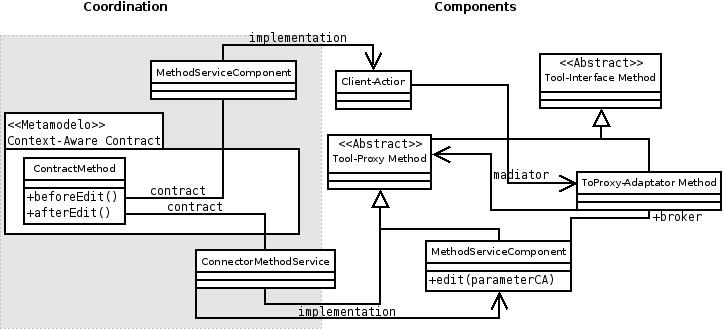
\includegraphics[width=5 in,totalheight=2.4 in]{Ch5/f4}
	\caption{\small \sl Diseño del modelo de integración} \label{contratos-patrones}
\end{center}
         \end{figure}

\begin{description}

\item[MétodoHerramineta\_Interfaz:] Como su nombre lo indica, esta es una clase
abstracta que define una interfaz común de los servicios de una Herramienta
provisto por \textbf{MétodoHerramienta\_Proxy}
y \textbf{MétodoToProxy\_Adaptador}

\item[MétodoToProxy\_Adaptador:] Esta es una clase concreta que implementa a un
intermediario manteniendo la referencia a la clase \textit{Método\_Proxy} para
encargarse de los pedidos recibidos. En tiempo de ejecución, esta entidad puede
indicar a \textbf{MétodoServiceComponente} que no hay contratos involucrados o
instrumentar una conexión entre \textbf{ConectorMétodosService} para que conecte
la clase real \textbf{MétodoServiceComponente} con el contrato
\textbf{ContractMétodo} en el que se encuentran las reglas de coordinación.

\item[MétodoHerramienta\_Proxy:] Es una clase abstracta que define la interfaz
que tienen en común \textbf{MétodoHerramientaToProxy\_Adaptador} y
\textbf{ConectorMétodoService}. La interfaz es heredada de
\textbf{MétodoHerramienta\_Interfaz} con el propósito de garantizar que ofrezca
la misma interfaz de \textbf{MétodoHerramientaToProxy\_Adaptador} con la cual un
cliente real debe interactuar (ej., un objeto que invoque el servicio de edición
de un Foro).

\item[EditServiceComponente:] Es la clase concreta  donde se encuentra la lógica
de la edición del Foro y la implementación concreta de los servicios originales
de Sakai.

\item[ConectorMétodoService:] Efectúa la conexión entre el contrato y los
objetos reales (en este caso \textbf{MétodoServiceComponente}) involucrados como
partes del contrato. De esta manera, no se requiere la creación o instanciación
de nuevos objetos para coordinar el mismo objeto real agregando o sacando otros
contratos. Esto es posible solamente con una nueva asociación a un nuevo
contrato y con la instanciación de una conexión con una instancia existente de
\textbf{ConectorMétodoService}. Esto significa que hay una sola instancia de
esta clase asociada con una instancia de \textbf{MétodoServiceComponente}.


\item [ContractMétodo:] Es la clase que cuya instancia genera un objeto de
coordinación que al ser notificado toma decisiones siempre que un pedido es
invocado a través de un objeto real.
Para los casos en que no haya contratos coordinando un objeto real, el diseño de
la figura \ref{contratos-patrones} puede ser simplificado y sólo las clases y
relaciones que no pasen por la zona del rectángulo gris son necesarias. La
introducción de un contrato implica la creación de las clases y relaciones
enmarcadas en la zona gris. La clase que implementa al contrato,  llamada
\textbf{ContractMétodo}, se encuentra representada dentro de la figura de un
paquete UML, llamado \textbf{Contratos Sensible al Contexto}, indicando su
pertenencia a un modelo subyacente descripto en la sección \ref{contrato}.
\end{description}

Este mecanismo de intercepción permite imponer otra funcionalidad en la
interacción entre componentes del llamante (por medio de su pedido) y del
llamado (a través de su respuesta). De esta manera, desde el aspecto tecnológico
se instrumenta la posibilidad de brindar un nuevo ``grado de libertad`` a los
servicios de Sakai, permitiendo establecer configuraciones propias de un DHD en
tiempo de ejecución.

Por lo expuesto, es válido reforzar la argumentación sobre las ventajas de esta
propuesta en comparación con las actuales soluciones tecnológicas basadas en
componentes y frameworks para la inyección y representación de servicios. A su
vez, se observa que el camino de su instrumentación es complejo debido a que se
deben generar (automáticamente) porciones de código y creación de nuevos
archivos código Java, a partir de los originales de la plataforma Sakai, que
deberán ser compilados y puestos en servicio para su operatividad. Cabe destacar
que los procesos de compilación y puesta en servicio de Sakai es efecutada una
sola vez, cualquier tipos de cambios y configuración serán impuestas a través
los contratos sensibles al contexto. 

La implementación de la coordinación de contratos en Sakai requiere del uso de
una herramienta específica para el dominio de aplicación (en este caso
aplicaciones e-learning) que modifica los archivos de código fuente Java que
implementan los servicios bases perteneciente al framework núcleo (similares a
los representados en esta sección), con el fin de incorporar la infraestructura
para trabajar con contratos de forma más o menos automática.

Para este propósito, se diseñó e implementó un prototipo experimental de una
herramienta llamada SwC ("Sakai with Contract") y un entorno de desarrollo que
permite instrumentar una metodología \cite{cacic,edutec} para la inclusión de
contratos en Sakai bajo la perspectiva de un DHD. El desarrollo de la
herramienta SwC está basada sobre el proyecto CED (Coordination Development
Environment)\footnote{CED: es el primer prototipo de una herramienta que
implementa el uso de la coordinación de contrato en aplicaciones Java. La
herramienta pertenece a ATX Software (www.atxsoftware.com);fue desarrollada
en Java y es de código abierto.} que implementa la coordinación de contrato a
través de un lenguaje llamado Oblog \cite{lenguajeoblog}. En este artículo no se
describen detalles técnicos de cómo la herramienta lleva a cabo la modificación
del código Java dentro de los distintos componentes de la arquitectura Sakai y
cuáles fueron las modificaciones puntuales efectuadas a partir de CED. 

%Las principales diferencias conceptuales entre CED y nuestra extensión parte de las propuestas enunciadas en la sección \ref{intro} y desarrolladas en la sección \ref{macroarquitectura} que ameritan un rediseño y agregados de módulos, algoritmos, interfaces, casos de uso, test, ejemplos, documentación, etc.


\section {Caso de estudio para la implementación de contratos} \label{caso de estudio}

En esta sección se presentará un caso de uso para ejemplificar las diferentes
etapas que se deben cumplimentar para lograr la inclusión de contratos en Sakai
bajo la perspectiva de los DHD, retomando la idea de incluir un contrato en los
servicios de edición de la herramienta Foro de Sakai.

Si bien consideramos importantes las observaciones realizadas sobre el por qué
de la necesidad de utilizar una metodología concreta para el diseño del contrato
referidas al lugar que ocupa dentro del flujo de ejecución de un Pe-lrn, qué
tipo de requerimientos satisface, cómo fueron relevados dichos requerimientos y
una especificación (en lo posible semi-formal) para su implementación, un
desarrollo más exhaustivo consta en otra publicación. Dicha metodología -llamada
UWATc- fue desarrollada en \cite{edutec}  para este mismo caso de estudio, y en
\cite{cacic} se amplían los detalles tecnológicos involucrados en su diseño. En
esta instancia UWATc brindará información sobre: cuáles son los servicios, en
qué clase (archivo Java) se encuentran representados (teniendo en cuenta el
flujo de ejecución) y cómo es configurado el contrato.

Nos centramos ahora en la última etapa del ciclo de vida de la configuración de
un espacio e-learning Web perteneciente al tiempo de compilación. En efecto, en
esta instancia el ingeniero de software cuenta con la información necesaria para
localizar los archivos de código fuente de la aplicación Sakai, los archivos de
configuración de los frameworks adicionales y demás configuraciones propias de
la herramienta para la inyección de los contratos.

Siguiendo  con el caso de estudio de las etapas anteriores, a continuación  se
muestra una porción de código Java correspondiente al código fuente original de
Sakai, en  donde se propone un método llamado \textbf{editMenssage}
correspondiente a la implementación del servicio edición de la herramienta Foro.
El siguiente fragmento de código fuente Java implementa una herencia de la clase
\textit{BaseDiscussionService} donde se encuentran las interfaces de los
servicios de edición correspondiente al núcleo del framework Sakai. 

\small \begin{verbatim}
import org.sakaiproject.discussion.api.DiscussionMessage; 
public class DiscussionService extends BaseDiscussionService{
public MessageEdit editMessage(MessageChannel channel, String id)‏{
return (MessageEdit) super.editResource(channel, id);}
\end{verbatim} \normalsize

Luego, a través de la herramienta SwC se crean archivos XML (similar a la
herramienta CED) para especificar las reglas del contrato que involucrarán
servicios implicados en el método \textit{editMensage} (Paso1). A continuación,
se ejecuta la generación automática de código para crear dos tipos de archivos
Java diferentes (Paso2). El primero (archivo 1) implementa las funcionalidades
que permitan las conexión con el Proxy (ej., \textit{MétodoHerramienta\_Proxy}
para nuestro caso de estudio); el segundo (archivo 2) implementa el conector
\textit{ConectorEditService} representado en la figura
\ref{contratos-patrones}. 

A continuación se muestran fragmentos de código que permiten una mejor
ilustración de las características adquiridas a partir de las modificaciones 
del código fuente de la aplicación Sakai a través de la herramienta.

\paragraph {Fragmentos del primer archivo - (archivo 1)}

\begin{enumerate}
 \item Se importan los paquetes correspondiente al framework de coordinación de
contratos (figura \ref{contratos-patrones}) y el framework context-aware (figura
\ref{contratoca})

\small \begin{verbatim}
package org.sakaiproject.discussion.impl; import java.util.*;
import cde.runtime.*; import obab.ca.*; // Framework context
public abstract class DiscussionService extends 
BaseMessageService implements 
DiscussionService,ContextObserver,EntityTransferrer,ForoInterface
\end{verbatim} \normalsize

\item  Métodos agregados por la herramienta para identificar las clases que van a ser interceptadas por el contrato.

\small \begin{verbatim}
protected CrdIProxy _proxy; 
private static Class _classId= Sakai.Discussion.class;
public static Class GetClassId() {return _classId;}
public CrdIProxy GetProxy() { return _proxy; }
public void SetProxy(Object p){if(p instanceof CrdIProxy && p instanceof 
DiscussionInterface) _proxy = (CrdIProxy)p; }
public void SetProxy(CrdIProxy p)  { _proxy = p; }
AccountInterface  GetProxy_Account(){if ( _proxy == null ) return null;  
return (DiscussionInterface) _proxy.GetProxy(_classId);}
\end{verbatim} \normalsize

\item Método que implementa la llamada del objeto cliente al Proxy

\small \begin{verbatim}
public long _getNumber(){new ComponentOperationEvent(this , "getNumber")_
.fireEvent(); return number;}
public messageEdit editMessage(MessageChannel channel,String id)‏{
new ComponentOperationEvent(this,"Edit").fireEvent();
return (MessageEdit) super.editResource(channel, id);}
\end{verbatim} \normalsize


\end{enumerate}

\paragraph {Fragmentos del segundo archivo - (archivo 2)}

\begin{enumerate}
\item Porción de código donde se importan las componentes de los frameworks, se
heredan las clases abstracta del los conectores y proxys. La clase del objeto
real \textit{MétodoService\_Componente}, según la figura
\ref{contratos-patrones}, se representa a través del atributo subject.

\small \begin{verbatim}
package org.sakaiproject; import java.util.*; 
import cde.runtime.*; import obab.ca.*;
public abstract class IDiscussionPartner extends 
CrdContractPartner implements CrdIProxy, DiscussiontInterface {
protected  Discussion subject;
\end{verbatim}\normalsize

\item Definición de los métodos abstractos para la conexión
(\textit{ConnectorMétodoService}, representada en la
figura \ref{contratos-patrones}), del contrato con el servicio.

\small \begin{verbatim}
public void SetProxy(Object p) {subject.SetProxy(p);}
protected Object GetSubject_Object() {return subject;}
public void ResetProxy() { subject.SetProxy(null);}
\end{verbatim}\normalsize


\item Métodos que permiten el acceso a los métodos que definen los servicios
(ej., métodos de la clase \textit{MétodoService_Componente})

\small \begin{verbatim}
protected Discussion GetSubjectDiscussion(){return (Discussion) subject;}
protected IDiscussionPartner GetNextPartner_Discussion(){
return (IDiscussionPartner)GetNextPartner(Discussion.GetClassId());}
\end{verbatim} \normalsize

\item Implementación por defecto de métodos definidos en la interfaces de los
servicios. A través del métodos \textit{GetSubjectDiscussion()}, detallado en el
punto anterior, se accede a los métodos creados por la herramienta en el primer
archivo.

\small \begin{verbatim}
public void messageEdit (double amount,Customer c)_
throws DiscussionException { IDiscussionPartner 
next = GetNextPartner_Discussion()
if (next != null) next.editMessage(amount,c); 
else GetSubjectDiscussion()._editMessage(amount,c);}
\end{verbatim} \normalsize

\item Implementaciones de los condicionales de la reglas de los contratos que se
encuentran en los archivos XML para configurarlos.

\small \begin{verbatim}
public CrdPartnerRules  messageEdit_rules(string texto,Student c) throws 
DiscussionException, CrdExFailure { return new CrdPartnerRules (this);}
\end{verbatim} \normalsize
\end{enumerate}

La generación de código automático a través de la herramienta presupone tener
ciertos niveles de conocimientos sobre: el lenguaje Java, aspectos de la
implementación del framework base Sakai y los frameworks que los componen; a
igual que experiencias en la compilación a través de Maven \footnote{Proyecto
maven: http://maven.apache.org/ref/2.0.4/maven-project/} de Sakai y las clases
modificadas-agregadas para el uso de contratos.

\section {Conclusión}

Fundamentados en el marco conceptual de los Dispositivos Hipermediales Dinámicos
para educación e investigación y en las actuales limitaciones observadas en las
plataformas e-learning sobre el grado de flexibilidad adaptativa en el sentido
de \cite{adaptativa} y \cite{kcomponent}), que pueda ser inducida por usuarios
expertos del dominio (ej., docentes) para el desarrollo de estrategias
didácticas efectivas para el logro de objetivos pedagógicos o investigativos 
planteados y, constando que dicha adaptabilidad no pueda ser enteramente resulta
por sistemas adaptativos inteligentes (ej., agentes, hipermedia adaptativa,
sistemas expertos, etc.), es que en este trabajo propusimos una implementación
de la teoría de coordinación de contrato en un framework específico sobre
sistemas colaborativos Web e-learning (correspondiente al proyecto Sakai)
brindando un modelo evolutivo conceptual y tecnológico. 
Partimos entonces, de las implementaciones de servicios y herramientas,
consideramos el agregado de componentes para la representación de cierta
información de contexto con aspectos context-aware para finalizar con la
incorporación de contratos para la coordinación de las interconexiones de los
servicios bases del framework original e-learning. De esta manera, el contrato
es una nueva primitiva prevista como una extensión de la noción de contratos de
B. Meyer \cite{Meyer} a la que se le adjudica el rol de coordinación de las
interacciones de los objetos.

El fin último de esta propuesta en desarrollo, se inscribe en brindar respuestas
tecnológicas efectivas a la necesidad de promover procesos educativos e
investigativos de interacción responsable entre los sujetos intervinientes en la
red sociotécnica del DHD, implementando la solución en los servicios cuya
prestaciones dependen -fuertemente- de reglas con estructuras volátiles cuyos
condicionales son influidos por el contexto (en el sentido de "Identificación
del contexto" desarrollado en el capítulo 5 \cite{libro} y manteniendo las
lineamientos sobre contexto fundados por P. Dourish \cite{contexto}). 

En este trabajo se propuso una implementación de la teoría de coordinación de
contrato en un framework específico sobre sistemas colaborativos Web e-learning
(correspondiente al proyecto Sakai). Se brindó un modelo evolutivo conceptual y
tecnológico, comenzando por las implementaciones de servicios y herramientas;
luego con el agregado de componentes para la representación de cierta
información de contexto con aspectos context-aware; finalizando con la
incorporación de contratos para la coordinación de las interconexiones de los
servicios bases del framework original e-learning. De esta manera, el contrato
es una nueva primitiva prevista como una extensión de la noción de contratos de
B. Meyer \cite{meyer} a la que se le adjudica el rol de coordinación de las
interacciones de los objetos.

Basados en nuestra visión de que las plataformas e-learning actuales carecen de
ciertos grados de flexibilidad adaptativa (en el sentido de \cite{adaptativa} y
\cite{kcomponent}), que pueda ser inducida por usuarios expertos del dominio
(ej., docentes, expertos en educación), para construir procesos educativos con
cierto grado de eficiencia. Donde, dicha adaptabilidad no pueda ser enteramente
resulta con sistemas adaptativos inteligentes (ej., agentes, hipermedia
adaptativa, sistemas expertos, etc.). Este requerimiento puntual hace referencia
a las necesidades de promover el tipo de solución que en este trabajo se
propone. Implementando la solución en los servicios cuya prestaciones dependen
-fuertemente- de reglas con estructuras volátiles cuyos condicionales son
influidos por el contexto (en el sentido de "Identificación del contexto"
desarrollado en el capítulo 5 \cite{libro} y manteniendo las lineamientos sobre
contexto fundados por P. Dourish \cite{contexto}). De esta manera se propone un
mecanismo para el diseño e implementación en tiempo de ejecución adaptada a un
tipo de aplicación e-learning Web.
